\documentclass[10pt,a4paper]{beamer}
\usepackage[backend=biber]{biblatex}
\addbibresource{bibliografiapaper}
\usepackage[utf8]{inputenc}
\usepackage[english]{babel}
\usepackage{amsmath}
\usepackage{amsfonts}
\usepackage{amssymb}
\usepackage{makeidx}
\usepackage{graphicx}
\usepackage{makecell}
\usepackage{verbatim}
\usefonttheme{professionalfonts} % fuentes de LaTeX
\usetheme{Szeged}
\usecolortheme{beaver}
\setbeamercovered{transparent}

\begin{document}
\title[Precise Weed and Maize Classification through Convolutional Neuronal Networks] %optional
{Precise Weed and Maize Classification through
Convolutional Neuronal Networks}
 
 
\author[C\'ordova Andrea, Barreno Mauricio and J\'acome Jos\'e] % (optional, for multiple authors)
{C\'ordova Andrea, Barreno Mauricio and J\'acome Jos\'e}
 
\institute[Universidad de las Fuerzas Armadas ESPE] % (optional)
{
  \inst{1}%
  Departamento de Energ\'ia y Mec\'anica\\
  Universidad de las Fuerzas Armadas ESPE
}
 
\date[Ecuador] % (optional)
{2nd IEEE Ecuador Technical Chapters Meeting, October 2017}
\logo{
\includegraphics[height=1.5cm]{espe.png}}
\frame{\titlepage}
%-----------------------------
\begin{frame}
\frametitle{Presentation Outline}
\tableofcontents
%\newpage
\end{frame}
%-----------------------------
\AtBeginSection[]
{
  \begin{frame}
    \frametitle{Table of Contents}
    \tableofcontents[currentsection]
  \end{frame}
}
\section{Introduction}
\begin{frame}
\frametitle{Introduction}
\textbf{Introduction}
\begin{itemize}
\item Maize(\textit{Zea mays}) is one of the most important crops of the world.
\item Weed can affect maize crop yield up to 5000 Kg/Ha.\footnote{ R. SU\'AREZ and J. P. Y. J. VALLADARES, “Distintos sistemas de escarda en ma\'iz forrajero,” \textit{Producciones agroganaderas: Gesti\'on eficiente
y conservaci\'on del Medio Natural. Actas de la XLV RC de la SEEP. Gij\'on}, 2005.} %Las malas hierbas en el maiz pueden afectan hasta 5000 Kg/Hectaria de produccion.
\item Robotics has had significant contributions to Precision Agriculture.%La robotica esta presentando grandes avances en la agricultura de precision.
\item Artificial Intelligence reached near-to-human precision.%Inteligencia artificial cada vez se acerca mas a la inteligencia humana.
\end{itemize}
\textbf{Purpose of the present study}
\begin{itemize}
\item Obtain samples to conform a dataset%Obtener muestras(imagenes) para conformar un dataset.
\item Segment samples%Segmentar las muestras.
\item Test accuracy in different network architectures of Convolutional Neural Networks for Maize and Weed Clasification %Probar diferentes arquitecturas de Redes Neuronales Convolucionales para entrenar la red.
\item Benchmark the best network architecture to analyze processing time %Hacer Benchmark en diferentes hardwares para analizar tiempos de procesamiento.
\item Optimize the network processing speed %Optimizar la red.
\end{itemize}
\end{frame}
%-----------------------------
\AtBeginSection[]
{
  \begin{frame}
    \frametitle{Table of Contents}
    \tableofcontents[currentsection]
  \end{frame}
}
\section{Used Hardware and Software}
\begin{frame}
\frametitle{Used Hardware and Software}
\textbf{Hardware}
\begin{enumerate}
\item Raspberry Pi 3.
\item Pi camera V2.1.
\item Nvidia graphic Card GTX950M.
\end{enumerate}
\textbf{Software}
\begin{enumerate}
\item OpenCV Library
\item Caffe framework
\item Ubuntu 16.04
\item PIXEL Distribution derived from Debian.
\end{enumerate}
\begin{figure}[hbtp]
%\caption{•}
\centering

\includegraphics[scale=0.3]{SoftHard.png}
\end{figure}

\end{frame}
%-----------------------------
\AtBeginSection[]
{
  \begin{frame}
    \frametitle{Table of Contents}
    \tableofcontents[currentsection]
  \end{frame}
}
\section{Image Processing}
\begin{frame}
\begin{itemize}
	\item Acquire  an RGB image through RPi Camera v2.1(Centered to the plant)
	
	\item Normalize Green Channel and then $S = 2*G - R - B$ \footnote{ P. Wang, Z. Meng, C. Luo, and H. Mei, “Path recognition for agricultural robot vision navigation under weed environment,” in \textit{7th International Conference on Computer and Computing Technologies in Agriculture (CCTA)}, no. Part I. Springer, 2013, pp. 242–248.
}
	\item OTSU Thresholding
	\item Detect contours and crop image to the contour 
	\item Mask image
	
\end{itemize}
\frametitle{Image Processing}
	\begin{figure}[h]
	\centering
	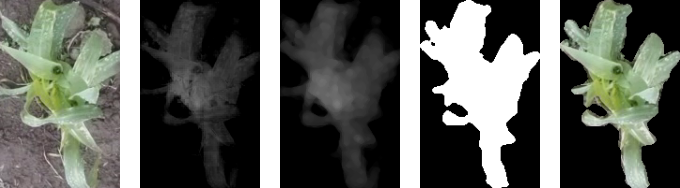
\includegraphics[width=3.5 in]{SegmentationPaper}
	\caption{Steps of image processing(Cropped image)}
	\label{figure4}
	\end{figure}
\end{frame}
%-----------------------------
\AtBeginSection[]
{
  \begin{frame}
    \frametitle{Table of
     Contents}
    \tableofcontents[currentsection]
  \end{frame}
}
\section{Dataset}
\begin{frame}
\frametitle{Dataset}
%{Dataset Description}
\begin{itemize}
\item Samples obtained in Pillaro-Tungurahua-Ecuador
\item Images obtained in its initial stage(3-7 leaves) . %La imagenes fueron obtenidas encampos de maiz en su estapa inicial,( plantas con 3 a 7 hojas) 
\item Rotated images every 30º to improve plant detection \footnote{ S. Sladojevic, M. Arsenovic, A. Anderla, D. Culibrk, and D. Stefanovic, “Deep neural networks based recognition of plant diseases by leaf image classification,” \textit{Computational intelligence and neuroscience}, vol. 2016, 2016.
}%Imagenes rotadas cada 30 grados para mejorar la deteccion de las planta.
\item 1/5 of the total images chosen randomly to validate training%1/5 del total de las imagenes al azar fueron usadas para la etapa de validacion
\end{itemize}
\begin{table}[h!]
\renewcommand{\arraystretch}{1.3}
\caption{Dataset distribution of each class}
\label{table:1}
\centering
\begin{tabular}{| c c c |} 
 \hline
 \textbf{Images} & \textbf{Maize} & \textbf{Weed}  \\ [1ex] 
 \hline
 Original  & 2835 & 880 \\ 
 Rotated & 34222 & 10762 \\ 
 Training & 25695 & 8560 \\
 Validation & 8325 & 2000 \\
 \hline
\end{tabular}
\end{table}
\end{frame}
\begin{frame}
\frametitle{Samples}
\begin{itemize}
\item Maize Plants \textit{(Zea maiz)}
\begin{figure}[h]
	\centering
	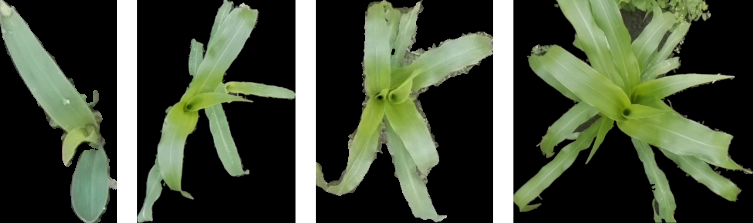
\includegraphics[width=3.5 in]{samplesmaize}
	%\caption{Normal architecture in a Convolutional Neural Network}
	\label{figure4}
	\end{figure}
	\item Weed Plants \textit{(Urtica Urens, Lysimachia vulgaris , Chenopodium \'album , Malva Capestri)} \footnote{COBA ROBALINO, José María. \textit{Monografía General del Cantón Píllaro.}} %Ortiga, Allpaquinua Cuchimalva, Forastera, Allpaquinua,  
\begin{figure}[h]
	\centering
	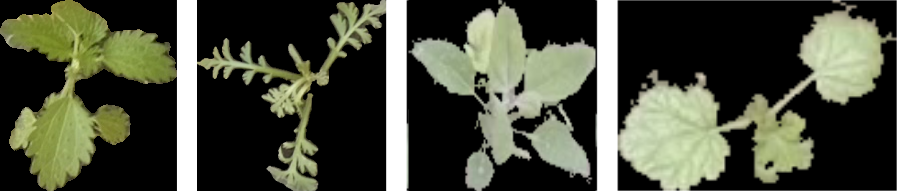
\includegraphics[width=3.5 in]{samplesweed}
	%\caption{Normal architecture in a Convolutional Neural Network}
	\label{figure4}
	\end{figure}
\end{itemize}
\end{frame}
%-----------------------------
\AtBeginSection[]
{
  \begin{frame}
    \frametitle{Table of Contents}
    \tableofcontents[currentsection]
  \end{frame}
}
\section{Convolutional Neural Networks}
\begin{frame}
\frametitle{Convolutional Neural Networks(CNN)}
\begin{itemize}
	\item Highly accurate method for image classification
	\item A class of deep, feed-forward artificial neural networks
	\item Tested on classification of plants, \footnote{B. Cheng and E. T. Matson, “A feature-based machine learning agent for automatic rice and weed discrimination.”} \footnote{ C. Potena, D. Nardi, and A. Pretto, “Fast and accurate crop and weed identification with summarized train sets for precision agriculture”
}
	\item Multiple architectures and applications
\end{itemize}
	\begin{figure}[h]
	\centering
	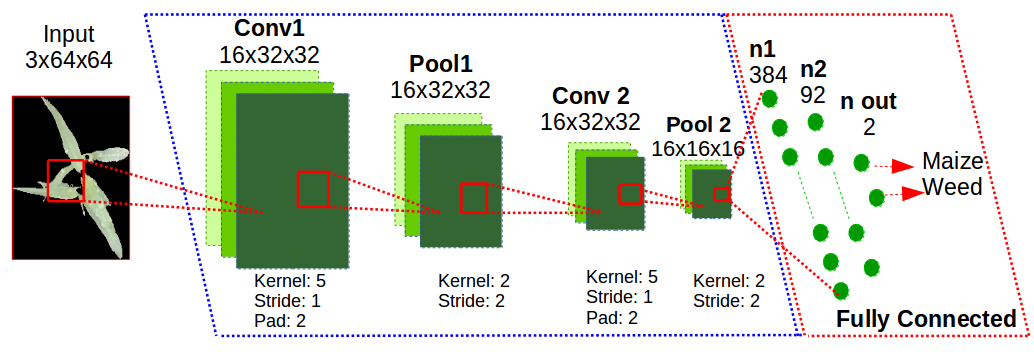
\includegraphics[width=3.5 in]{arquitectura}
	\caption{Normal architecture in a Convolutional Neural Network}
	\label{figure4}
	\end{figure}
\end{frame}
\AtBeginSection[]
{
  \begin{frame}
    \frametitle{Table of Contents}
    \tableofcontents[currentsection]
  \end{frame}
}
\section{Tested Architectures}
\begin{frame}
\frametitle{Tested Architectures}
\begin{itemize}
	\item LeNET and AlexNet(Caffe Zoo Model) \
	\item cNET and sNET \footnote{ C. Potena, D. Nardi, and A. Pretto, “Fast and accurate crop and weed identification with summarized train sets for precision agriculture”
}
	\item 3000 iterations in each training
\end{itemize}
\begin{table}[h!]
\centering
\renewcommand{\arraystretch}{1.2}
\caption{Comparison of the 4 types of CNN in training the dataset}
\label{table:2}
\begin{tabular}{|l c c c c|} 
 \hline
 \textbf{Parameters }& \textbf{LeNet} & \textbf{AlexNet} & \textbf{cNET} & \textbf{sNET} \\ [0.75ex] 
 \hline
 Input size of images & 32x32 & 64x64 & 64x64 & 64x64 \\ 
 Layers numbers & 9 & 11 & 8 & 4\\
 Number of parameters & 652500 & 20166688 & 6421568 & 135872 \\ 
 Accuracy(\%) & 86.48 & 93.86 & 96.4 & 80.4 \\
 Loss(\%) & 32.80 & 15.32 & 13.72 & 15.32 \\ [1ex] 
 \hline 
\end{tabular}
\end{table}
\end{frame}
%-----------------------------
\AtBeginSection[]
{
  \begin{frame}
    \frametitle{Table of Contents}
    \tableofcontents[currentsection]
  \end{frame}
}
\section{Tuning cNET}
\begin{frame}
\frametitle{cNET Performance}
\begin{enumerate}
\item cNET can be improved by decreasing the number of filters
\item Images can be batched and also Caffe can be multithreaded
\item Both nets were trained with 9000 iterations
\end{enumerate}
\begin{table}[h]
\centering
\renewcommand{\arraystretch}{1.2}
\caption{Comparison between cNET of 16 and 64 filters}
\label{table:3}
\begin{tabular}{|l c c |} 
 \hline
 \textbf{Parameters} & \textbf{cNET 16 filters} & \textbf{cNET 64 filters} \\ [0.75ex] 
 \hline
 Number of parameters & 1651376 & 6421568 \\ 
 Accuracy(\%) & 97.26 & 96.40 \\
 Loss(\%) & 8.39 & 13.72 \\ [1ex] 
 \hline 
\end{tabular}
\end{table}
\end{frame}
%-----------------------------
\AtBeginSection[]
{
  \begin{frame}
    \frametitle{Table of Contents}
    \tableofcontents[currentsection]
  \end{frame}
}
\section{Estimated performance of cNET 16 filters}
\begin{frame}
\frametitle{Estimated performance of cNET 16 filters}
\begin{itemize}
	\item A test dataset with 202 images of each class was used
	\item 18 plants can be found in a single image approximately to be classified
\end{itemize}
\begin{table}[h!]
\centering
\renewcommand{\arraystretch}{1.2}
\caption{Test of complete image classification in FPS}
\label{table:6}
\begin{tabular}[c c c c]{|p{1.8 cm} p{1.5cm} p{2.1cm} p{2.3cm}|} 
 \hline
 \textbf{Parameter} &\textbf{GPU } & \textbf{CPU} & \textbf{Raspberry Pi} \\ 
 \hline
  \textbf{Method} &\textbf{One Core} & \textbf{Multithreading} & \textbf{Multithreading} \\ 
 \hline
 Time(s) & 0.0171 & 0.196 & 2.714 \\ [0.95ex]
 FPS & 58.47 & 5.08 & 0.36 \\ [0.95ex]
 \hline
\end{tabular}
\end{table}
\end{frame}
%--------------
\AtBeginSection[]
{
  \begin{frame}
    \frametitle{Table of Contents}
    \tableofcontents[currentsection]
  \end{frame}
}
\section{Conclusion}
\begin{frame}
\frametitle{Conclusion}
\begin{itemize}
\item cNET showed the best results in classification of maize and weed
\item The reduction of the number of filters decreased the processing time and increased the network accuracy 
\item GPU showed the best results, but with Multithreading and Batching CPU and Raspberry Pi can improve its processing time
\item Due to the limitations of the Raspberry Pi, it can't be used to classify in real time, but a Neural Module(such as Intel Movidius) can improve that result
\end{itemize}
\end{frame}
%--------------
\large
\begin{frame}
%\frametitle{The Propose of the present study}
\begin{center}
Thanks!
\end{center}
\end{frame}

%-----------------------------
%\bibliographystyle{plain}
%\bibliography{bibliografiapaper}
\end{document}
